\documentclass[11pt]{article}

% CAISc 2026 style
\usepackage{caisc_2026}

\usepackage[utf8]{inputenc}
\usepackage[T1]{fontenc}
\usepackage{times}
\usepackage{microtype}
\usepackage{graphicx}
\usepackage{booktabs}
\usepackage{caption}
\usepackage{subcaption}
\usepackage{amsmath, amssymb}
\usepackage{enumitem}
\usepackage{hyperref}
\usepackage{xcolor}
\usepackage{makecell}
\usepackage{pifont}
\newcommand{\cmark}{\ding{51}}
\newcommand{\xmark}{\ding{55}}
\usepackage{tikz}
\usetikzlibrary{arrows.meta, positioning, shapes.geometric, fit, backgrounds, calc}

\definecolor{ink}{HTML}{0F1B2D}
\definecolor{accent}{HTML}{1B4D3E}

\hypersetup{
  colorlinks=true,
  linkcolor=ink,
  citecolor=accent,
  urlcolor=accent
}

\title{World Model-Inspired Agentic Reasoning with Compounding Memory:\\
  A Staged Architecture for Industrial Fermentation}

\author{
  Anonymous Author(s) \\
  Affiliation \\
  \texttt{email}
}

\begin{document}

\maketitle

\begin{figure}[h]
\centering
\resizebox{\linewidth}{!}{%
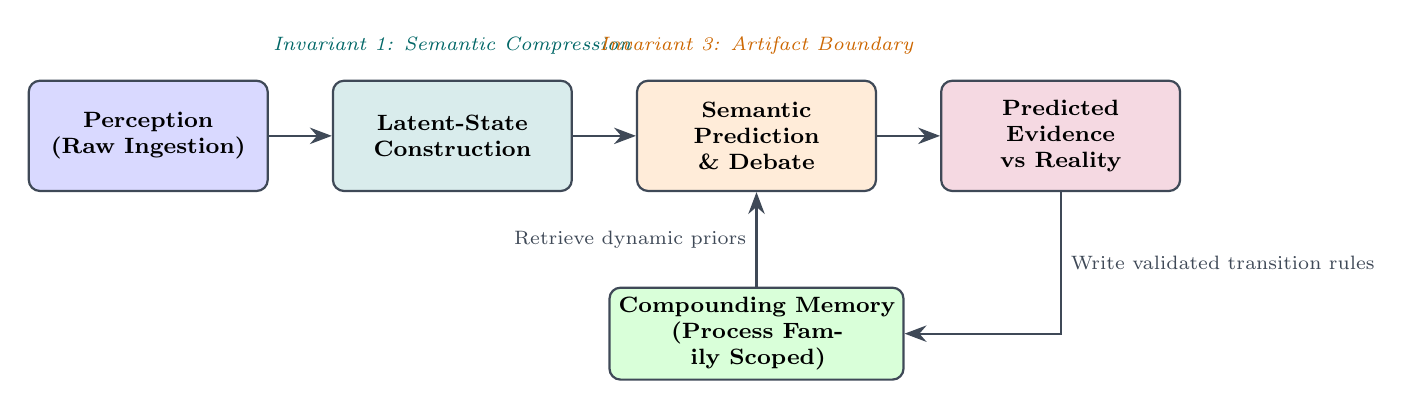
\begin{tikzpicture}[
  node distance=0.8cm,
  box/.style={rectangle, draw=ink!80, thick, rounded corners, text width=2.8cm, text centered, minimum height=1.4cm, font=\footnotesize\bfseries},
  arrow/.style={-{Stealth[scale=1.2]}, thick, ink!80}
]
  \node[box, fill=blue!15] (data) {Perception\\(Raw Ingestion)};
  \node[box, fill=teal!15, right=of data] (char) {Latent-State\\Construction};
  \node[box, fill=orange!15, right=of char] (agent) {Semantic Prediction\\\& Debate};
  \node[box, fill=purple!15, right=of agent] (insight) {Predicted Evidence\\vs Reality};
  
  \draw[arrow] (data) -- (char);
  \draw[arrow] (char) -- (agent);
  \draw[arrow] (agent) -- (insight);
  
  \node[box, fill=green!15, text width=3.5cm, minimum height=1cm, below=1.2cm of agent] (memory) {Compounding Memory\\(Process Family Scoped)};
  
  \draw[arrow] (insight.south) |- (memory.east) node[pos=0.25, right, font=\scriptsize] {Write validated transition rules};
  \draw[arrow] (memory.north) -- (agent.south) node[midway, left, font=\scriptsize] {Retrieve dynamic priors};
  
  \node[above=0.2cm of char, font=\scriptsize\itshape, text=teal!80!black] {Invariant 1: Semantic Compression};
  \node[above=0.2cm of agent, font=\scriptsize\itshape, text=orange!80!black] {Invariant 3: Artifact Boundary};
  
\end{tikzpicture}%
}
\caption*{Graphical Abstract: The FermDocs architecture is inspired by world-model cognition — compressing raw sensor streams into semantic latent states, utilizing multi-agent debate for falsifiable causal chains, and reinforcing a cross-run memory. The system is fully open-source.}
\end{figure}

\begin{abstract}
Most multi-agent LLM systems for scientific reasoning generate textually plausible explanations directly from raw observations. We argue this paradigm is structurally limited and that the path forward is a world model-inspired architecture: one that compresses noisy observations into stable latent states, articulates falsifiable causal chains, and evaluates consequences against observed reality. We present FermDocs, a fully open-source, staged architecture for industrial fermentation hypothesis generation that cognitively decomposes reasoning into perception, latent-state construction, observational interpretation, and causal hypothesis testing. While FermDocs does not yet execute numerical forward simulations, it performs \emph{semantic state-transition reasoning}—forcing agents to declare the necessary downstream consequences of their hypotheses and verifying them against the bundle evidence. Crucially, FermDocs introduces a \emph{cumulative cross-run memory} scoped by a closed-vocabulary domain identifier. By systematically digesting multi-agent critiques into persistent transition rules, the system's domain-specific priors accumulate across successive experiments, enabling each run to build on prior runs rather than starting from scratch. We position FermDocs as a world model-inspired agentic system for bioprocessing, detail how its structural invariants (schema-enforced provenance, domain-scoped memory, and artifact separation) make it uniquely effective, and present a two-phase evaluation methodology to rigorously assess its reasoning capabilities.
\end{abstract}

% =========================================================
\section{Introduction}
% =========================================================

Industrial fermentation generates exactly the kind of data that breaks
single-pass language models. A single penicillin or yeast run produces
tens of thousands of timestamped measurements across dissolved oxygen,
pH, biomass, substrate, off-gas, temperature, agitation, and feed
profiles, accompanied by Excel batch sheets, narrative operator logs in
PDF format, and process control system exports with inconsistent header
conventions. When a bioprocess engineer asks why a particular run lost
productivity, the answer requires integrating evidence across these
modalities, recognizing when an apparent anomaly is a measurement
artifact rather than a biological process event, distinguishing observation from
inference, and grounding every claim in a specific cell of a specific
file. In regulated bioprocess environments, reviewers cannot accept
explanations that are merely plausible; they require explanations whose
provenance is strictly traceable to source data.

Contemporary multi-agent scientific reasoning systems—such as the AI Co-Scientist~\citep{aicoscientist}, Robin~\citep{robin}, BioDiscoveryAgent~\citep{biodisco}, and SciAgents~\citep{sciagents}—attempt to solve complex reasoning tasks by providing LLMs with tools and chaining their textual outputs. However, these systems fundamentally operate by generating \emph{plausible textual explanations} directly from observations. They lack stable latent states, temporal consistency, and process-level transition mechanics. A language model looking at a time-series drop in dissolved oxygen and textually guessing ``oxygen limitation'' is engaging in pattern matching, not scientific reasoning.

We argue that the path forward for complex engineering domains is not more agents or larger contexts, but a world model-inspired architecture: compressing noisy observations into stable latent states, hypothesizing causal transitions, and evaluating consequences against observed reality. World models in the technical sense map raw observations to a semantic latent state, hypothesize a causal perturbation, and evaluate the downstream evidence implied by that perturbation. FermDocs is inspired by this paradigm: it implements the cognitive decomposition (perception, latent-state compression, causal hypothesis, downstream verification) without yet implementing the learned dynamics.

\begin{figure}[htbp]
\centering
\resizebox{\linewidth}{!}{%
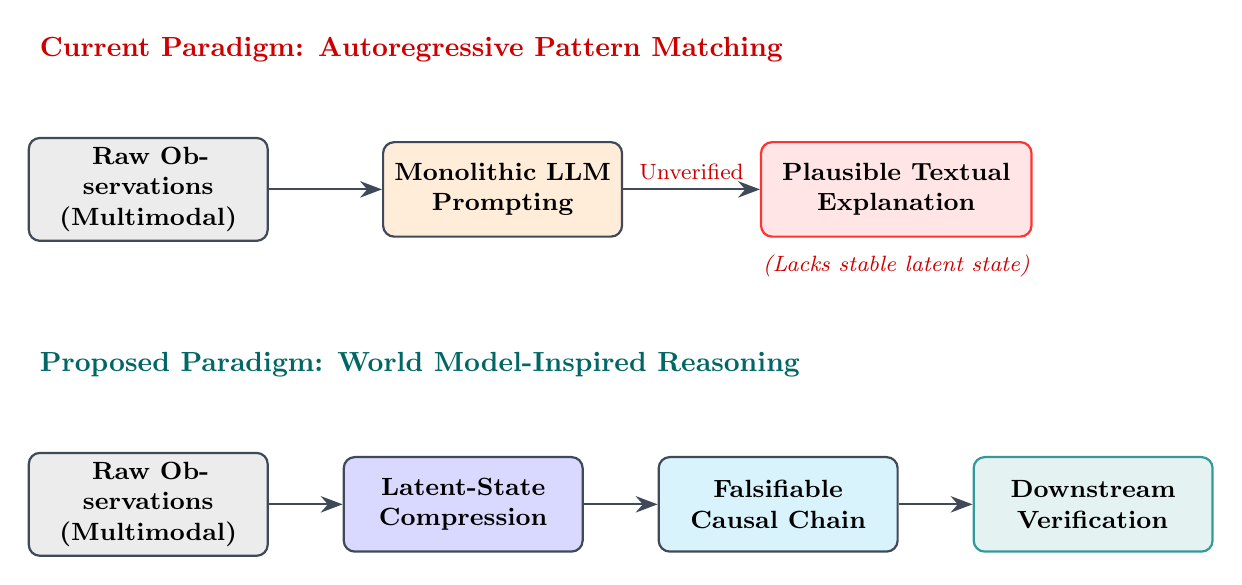
\begin{tikzpicture}[
  box/.style={rectangle, draw=ink!80, thick, rounded corners, text width=2.8cm, text centered, minimum height=1.2cm, font=\small\bfseries},
  alert/.style={rectangle, draw=red!80, thick, fill=red!10, rounded corners, text width=3.2cm, text centered, minimum height=1.2cm, font=\small\bfseries},
  good/.style={rectangle, draw=teal!80, thick, fill=teal!10, rounded corners, text width=2.8cm, text centered, minimum height=1.2cm, font=\small\bfseries},
  arrow/.style={-{Stealth[scale=1.2]}, thick, ink!80}
]

  % Top row: Current Paradigm
  \node[anchor=south west, font=\bfseries\normalsize, text=red!80!black] at (-1.5, 1.5) {Current Paradigm: Autoregressive Pattern Matching};
  
  \node[box, fill=gray!15] (raw1) at (0,0) {Raw Observations\\(Multimodal)};
  \node[box, fill=orange!15] (llm) at (4.5,0) {Monolithic LLM\\Prompting};
  \node[alert] (text) at (9.5,0) {Plausible Textual\\Explanation};
  
  \draw[arrow] (raw1) -- (llm);
  \draw[arrow] (llm) -- (text) node[midway, above, font=\footnotesize, text=red!80!black] {Unverified};
  \node[below=0.1cm of text, font=\footnotesize\itshape, text=red!80!black] {(Lacks stable latent state)};

  % Bottom row: World-Model Paradigm
  \node[anchor=south west, font=\bfseries\normalsize, text=teal!80!black] at (-1.5, -2.5) {Proposed Paradigm: World Model-Inspired Reasoning};
  
  \node[box, fill=gray!15] (raw2) at (0,-4) {Raw Observations\\(Multimodal)};
  \node[box, fill=blue!15] (latent) at (4,-4) {Latent-State\\Compression};
  \node[box, fill=cyan!15] (sim) at (8,-4) {Falsifiable\\Causal Chain};
  \node[good] (verify) at (12,-4) {Downstream\\Verification};
  
  \draw[arrow] (raw2) -- (latent);
  \draw[arrow] (latent) -- (sim);
  \draw[arrow] (sim) -- (verify);
  
\end{tikzpicture}%
}
\caption{The architectural gap in current scientific reasoning systems. Contemporary systems (top) compress reasoning into a single autoregressive generation step, producing plausible but structurally ungrounded explanations. A world model-inspired approach (bottom) decomposes this into latent-state compression, causal hypothesis generation, and explicit downstream verification.}
\label{fig:paradigm_gap}
\end{figure}
 

To bridge this gap, we present \textbf{FermDocs}, a fully open-source, publicly available multi-agent architecture designed explicitly around cognitive decomposition. FermDocs replaces the traditional ``LLM + tools + chain-of-thought'' paradigm with a pipeline that rigorously separates perception (ingestion), latent-state construction (characterization), observational interpretation (diagnosis), and causal reasoning (hypothesis debate). 

Importantly, while FermDocs does not currently execute numerical forward simulations (such as solving ODEs for biomass growth), it implements \emph{semantic state-transition prediction}. The architecture forces agents to hypothesize causal transitions (e.g., A leads to B) and empowers a Critic agent to evaluate whether the expected downstream markers of that transition actually materialized in the data.

Crucially, FermDocs features a \emph{compounding cross-run memory}. Unlike standard retrieval-augmented generation (RAG) systems that simply retrieve additive text based on vector similarity, the FermDocs memory layer persists validated critiques and state-transition lessons indexed by a strict, closed-vocabulary \texttt{process\_family} identifier (e.g., \emph{Saccharomyces cerevisiae} aerobic fed-batch). As the system analyzes more runs, its internal priors accumulate, continuously improving its predictive accuracy and reasoning depth over time.

This paper details the FermDocs architecture and its three core structural invariants:
\begin{itemize}[leftmargin=*]
    \item \textbf{Invariant 1 (Schema-Enforced Citation).} Every hypothesis claim carries a non-empty list of citations to upstream findings, observations, or narrative anchors, enforced at the schema validation layer before any downstream agent reads the claim. This directly addresses the failure mode PiFlow~\citep{piflow} identifies as central to contemporary multi-agent hypothesis systems—claims that lack clear links to supporting or refuting evidence—not by improving prompts but by making unlinked claims structurally invalid at object construction time; downstream agents cannot consume a hypothesis whose citation field has not been satisfied.
    
    \item \textbf{Invariant 2 (Domain-Scoped Memory).} Cross-run lessons are keyed on a closed-vocabulary \texttt{process\_family} identifier validated at the protocol boundary. A query without a domain key raises an exception at validation time. This addresses the Rupprecht review's~\citep{rupprecht2026} explicit observation that only one of nine surveyed chemical-engineering MAS uses a fixed domain ontology—extending the design philosophy from knowledge representation into memory routing, and making cross-domain lesson contamination structurally impossible rather than discouraged in prompts.
    
    \item \textbf{Invariant 3 (Observational--Causal Artifact Separation).} Observational reasoning (what happened, what trended) and causal reasoning (why, by what mechanism) are separated at the typed JSON artifact boundary between stages, not within the prompt of any single agent. This prevents the failure mode where causal speculation contaminates evidence summaries—a mode endemic to monolithic LLM reasoning that no surveyed system in either the AI-for-science or chem-eng MAS literatures structurally prevents.
\end{itemize}

We position this architecture against the chemical-engineering MAS literature in Section~\ref{sec:related}. We provide a deep dive into the system mechanics, explaining exactly how it is built and why this specific decomposition is so effective in Section~\ref{sec:system}. Finally, we define a structured, two-phase evaluation methodology designed to capture the nuances of latent-state reasoning in Section~\ref{sec:evaluation}. 

% =========================================================
\section{Related work}
\label{sec:related}
% =========================================================

\paragraph{Multi-agent scientific reasoning and world-model inspiration.} 
The AI Co-Scientist~\citep{aicoscientist} established the contemporary template for multi-agent hypothesis generation through Elo-based tournament refinement. However, the recent PiFlow framework~\citep{piflow} diagnoses the core failure mode of this family: hypotheses produced by such systems often ``lack clear direction, leading to uncertainty in establishing clear links between hypotheses and their supporting or refuting evidence.'' 
Separately, the world-models literature~\citep{lecun2022,ha2018,hafner2023} emphasizes reasoning through learned state evolution rather than reactive generation. FermDocs draws inspiration from this paradigm without claiming implementation parity. By compressing observations into a stable latent space and forcing agents to articulate downstream consequences, FermDocs transforms multi-agent debate from a textual plausibility contest into an evaluation of expected downstream evidence against reality.

\paragraph{Multi-agent systems in chemical engineering.} 
The Rupprecht review~\citep{rupprecht2026} surveys nine systems applied to process engineering, identifying six open challenges. Directed cyclic graphs dominate because chemical engineering workflows have inherent feedback loops. Pajak and colleagues~\citep{pajak} use a multi-agent debate among agents representing different objectives (cost, emissions) for operational decision-making, while Zeng and colleagues~\citep{zeng} apply multi-agent collaboration to process optimization. Of the nine systems surveyed, exactly one uses a fixed domain-specific ontology rather than a dynamically-extracted one. Our closed-vocabulary \texttt{process\_family} enum addresses this unmet need directly, extending the design philosophy from knowledge representation into \emph{routing} and \emph{memory scoping}. Rupprecht et al. identify six open challenges for chemical-engineering MAS: tailored architectures, tool integration as a first-class concern, structured database integration, domain-ontology-backed knowledge representation, human integration with both static and dynamic checkpoints, and domain-specific foundation models. FermDocs addresses five of these directly through the architecture described in Section 3: a directed-cyclic-graph hypothesis stage within a staged pipeline (architecture), bounded tool surfaces with structured output contracts (tools), typed bundle artifacts plus a managed memory backend (databases), the closed-vocabulary \texttt{process\_family} enum (ontology), and HITL pause/resume with state preservation (human integration). The sixth challenge—domain-specific foundation models—remains future work, as it does for the broader field. To our knowledge, no system in the surveyed literature addresses more than two of these challenges simultaneously.

Table~\ref{tab:comparison} compares FermDocs against representative systems from both the AI-for-science and chemical-engineering multi-agent literatures. The columns correspond to the structural commitments this paper argues are load-bearing for grounded scientific reasoning. Systems are evaluated on whether each commitment is structurally enforced (\cmark), absent (\xmark), or implemented through a related but not equivalent mechanism (described in the cell). FermDocs is the only system in the comparison set that combines schema-enforced citation, closed-vocabulary domain scoping, cross-run memory, and source-data provenance. It explicitly does not implement learned forward dynamics — this is the JEPA gap that Section~\ref{sec:discussion} acknowledges directly.

\begin{table}[htbp]
\centering
\small
\caption{Structural properties of selected multi-agent scientific reasoning systems. \cmark~indicates the property is structurally enforced; \xmark~indicates it is absent; Partial indicates a related but not equivalent capability. FermDocs is the only surveyed system that combines schema-enforced citation, closed-vocabulary domain scoping, cross-run memory, and source-data provenance. The honest \xmark~on forward dynamics reflects the JEPA gap acknowledged in Section~\ref{sec:discussion}.}
\label{tab:comparison}
\resizebox{\linewidth}{!}{%
\begin{tabular}{lccccc}
\toprule
System & \makecell{Schema\\citation} & \makecell{Closed-vocab\\scoping} & \makecell{Cross-run\\memory} & \makecell{Source-data\\provenance} & \makecell{Forward\\dynamics} \\
\midrule
AI Co-Scientist \citep{aicoscientist} & \xmark & \xmark & \xmark & lit.\ only & \xmark \\
Robin \citep{robin} & \xmark & \xmark & \xmark & assay only & \xmark \\
BioDiscoveryAgent \citep{biodisco} & \xmark & \xmark & \xmark & \xmark & \xmark \\
SciAgents \citep{sciagents} & \xmark & \xmark & \xmark & \xmark & \xmark \\
El Agente \citep{elagente} & \xmark & \xmark & \xmark & \xmark & \xmark \\
Pajak et al.\ \citep{pajak} & \xmark & \xmark & \xmark & simulator & \cmark~(Aspen) \\
Zeng et al.\ \citep{zeng} & \xmark & \xmark & \xmark & simulator & \cmark~(IDAES) \\
Taskiran et al.\ \citep{taskiran} & \xmark & \cmark & \xmark & \xmark & \xmark \\
\midrule
\textbf{FermDocs (ours)} & \textbf{\cmark} & \textbf{\cmark} & \textbf{\cmark} & \textbf{\cmark} & \textbf{\xmark} \\
\bottomrule
\end{tabular}%
}
\end{table}

The pattern is not that FermDocs is uniformly stronger than every compared system on every axis. Pajak et al.\ and Zeng et al.\ integrate first-principles process simulators (Aspen HYSYS and IDAES respectively), giving them forward-dynamics capabilities FermDocs lacks. Taskiran et al.\ implements a fixed domain ontology, the only such system in the Rupprecht survey besides FermDocs. The contribution of the present work is not winning every axis but combining schema-enforced citation, domain-scoped compounding memory, and observational--causal artifact separation at the type system rather than the prompt — a combination no surveyed system exhibits.


\paragraph{Cross-Run Memory and Debate.} 
Multi-agent debate improves factual accuracy and reasoning quality over single-agent baselines~\citep{du2023,liang2023}. However, self-critique by the same underlying model is unreliable and can introduce false negatives~\citep{huang2024}, a symptom of broader structural failures in multi-agent reasoning systems~\citep{cemri2025}. We address this through asymmetric information design, coupled with a persistent memory layer. When a debate concludes, the system digests the verified criticisms into persistent state-transition rules. This allows the system's reasoning capabilities to compound over time, dynamically evolving its priors based on empirical outcomes rather than remaining a static retrieval system.

% =========================================================
\section{System architecture: A World Model-Inspired Decomposition}
\label{sec:system}
% =========================================================

\begin{figure}[htbp]
\centering
\resizebox{\linewidth}{!}{%
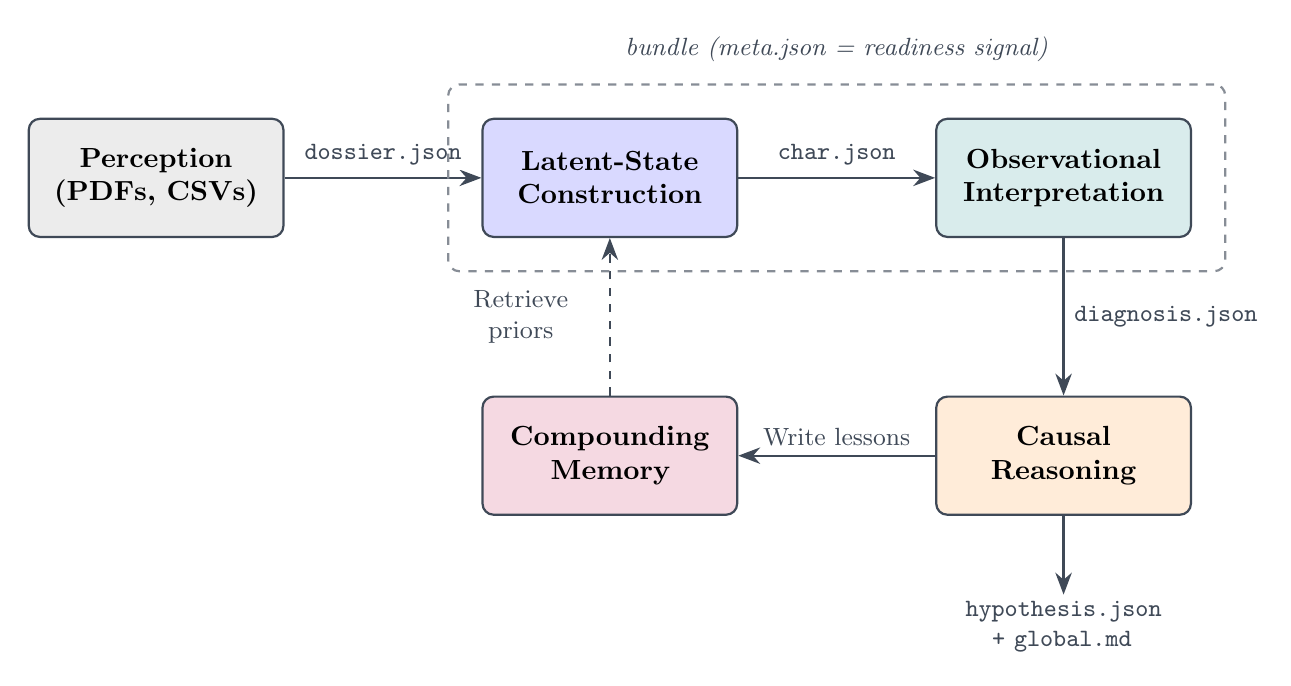
\begin{tikzpicture}[
  node distance=2.2cm and 2.5cm,
  stage/.style={rectangle, draw=ink!80, thick, text width=3cm, text centered, rounded corners, minimum height=1.5cm, font=\normalsize\bfseries},
  artifact/.style={fill=white, font=\ttfamily\small, inner sep=2pt},
  arrow/.style={-{Stealth[scale=1.2]}, thick, ink!80}
]
  \node[stage, fill=gray!15] (raw) {Perception\\ (PDFs, CSVs)};
  \node[stage, fill=blue!15, right=of raw] (ingest) {Latent-State\\ Construction};
  \node[stage, fill=teal!15, right=of ingest] (diagnose) {Observational\\ Interpretation};
  
  \node[stage, fill=orange!15, below=2cm of diagnose] (hypothesis) {Causal\\ Reasoning};
  \node[stage, fill=purple!15, left=of hypothesis] (memory) {Compounding\\ Memory};
  
  \draw[arrow] (raw) -- (ingest) node[midway, artifact, yshift=0.3cm] {dossier.json};
  \draw[arrow] (ingest) -- (diagnose) node[midway, artifact, yshift=0.3cm] {char.json};
  
  \draw[arrow] (diagnose) -- (hypothesis) node[midway, artifact, xshift=1.3cm] {diagnosis.json};
  \draw[arrow] (hypothesis.south) -- ++(0,-1) node[below, artifact, text width=3cm, text centered] {hypothesis.json\\+ global.md};
  
  \draw[arrow] (hypothesis.west) -- (memory.east) node[midway, above, font=\small] {Write lessons};
  \draw[arrow, dashed] (memory.north) -- (ingest.south) node[midway, left, font=\small, text width=2cm, text centered] {Retrieve\\priors};

  % Adjust bundle bounding box
  \node[draw=ink!50, dashed, thick, rounded corners, inner sep=12pt, fit=(ingest) (diagnose)] (bundle) {};
  \node[above=0.15cm of bundle, font=\small\itshape, text=ink!80] {bundle (meta.json = readiness signal)};
\end{tikzpicture}%
}
\caption{The system operates as a four-stage pipeline inspired by world-model cognitive decomposition. Each stage emits a typed JSON artifact. The boundaries between stages are not code method calls, but persisted files on disk. The hypothesis stage fetches and writes cross-run lessons through a \texttt{MemoryBackend} protocol, enabling priors to accumulate across runs within each process family.}
\label{fig:pipeline}
\end{figure}

The system processes raw fermentation reports through four sequential stages (Figure~\ref{fig:pipeline}), explicitly inspired by world-model cognitive decomposition (perception, latent-state construction, causal hypothesis, downstream verification). Each stage takes a typed input artifact, performs its work, and emits a typed output artifact. The boundaries between stages are persisted JSON files validated by typed schema contracts. We implement these schema contracts in Pydantic; any equivalent typed-schema system would suffice. 

This decomposition is the primary reason the architecture is highly effective. By preventing the system from collapsing all tasks into a single context window, FermDocs avoids attention dilution. An LLM tasked with parsing a PDF, finding anomalies, and hypothesizing biological causes simultaneously will inevitably hallucinate. FermDocs restricts the action space at every step, leveraging deterministic code where mathematics are sufficient, and reserving LLMs strictly for semantic interpretation.

\subsection{Perception (Ingestion \& Parsing)}

The ingest stage acts as the system's sensory apparatus. It parses CSV, Excel, and PDF inputs, leveraging tools like \texttt{docling} for robust PDF segmentation and \texttt{pint} for deterministic unit normalization (e.g., safely standardizing Fahrenheit to Celsius or differing volume metrics to liters). 

This stage produces a \texttt{dossier.json} containing noisy observations with full provenance back to source files, sheets, cells, and pages. Critically, the dossier carries a canonical \texttt{process\_family} identifier drawn from a closed vocabulary defined in YAML (e.g., \texttt{aerobic\_fed\_batch\_glucose} under \emph{Saccharomyces cerevisiae}). If the system does not recognize the family, it routes to an `unknown` generic catalog, preventing hallucinated domain logic.

\subsection{Latent-State Construction (Characterization)}

World models do not reason directly over raw sensor streams; they require the compression of noisy observations into stable semantic latent states. FermDocs adopts this design principle without implementing the learned compression itself, achieving it through strict, deterministic characterization.

This stage executes a predefined metric catalog. It algorithmically detects metadata anomalies such as equipment changes, header inconsistencies, scale changes, or $h_0$ (time zero) outliers. It computes process and product KPIs specific to the \texttt{process\_family}. 

By emitting typed findings with globally unique, stable identifiers (e.g., \texttt{F-0014}), this stage abstracts the raw data into a latent-state space. For example, instead of passing thousands of DO (Dissolved Oxygen) data points to the LLM, the characterization stage passes a single, mathematically verified finding: ``Sustained DO drop below 20\% between hours 14 and 18.'' This compression is the defining prerequisite of world model architectures and is what enables the downstream causal reasoning to operate on stable semantic states rather than noisy sensor streams.

\subsection{Observational Interpretation (Diagnosis)}

The diagnosis stage is a bounded ReAct~\citep{react} (Reason + Act) agent loop that interprets the latent state space. Its job is to figure out \emph{what} happened, but deliberately not \emph{why} it happened. 

It consumes the characterization output and utilizes a strict set of internal tools to query the data. It produces typed claims: \texttt{FailureClaim} (process deviations), \texttt{TrendClaim} (sustained directional changes), and \texttt{AnalysisClaim} (cross-variable correlations). 

To ensure invariant enforcement, every single claim validated by the schema contract \emph{must} cite at least one upstream finding identifier. This strict provenance enforcement prevents the LLM from hallucinating claims without anchoring them to the established latent state. If an agent emits a claim without a valid \texttt{F-XXXX} citation, the framework intercepts the output, blocks it, and forces a retry.

\subsection{Causal Reasoning \& Downstream Verification (Hypothesis Stage)}

\begin{figure}[htbp]
\centering
\resizebox{0.75\linewidth}{!}{%
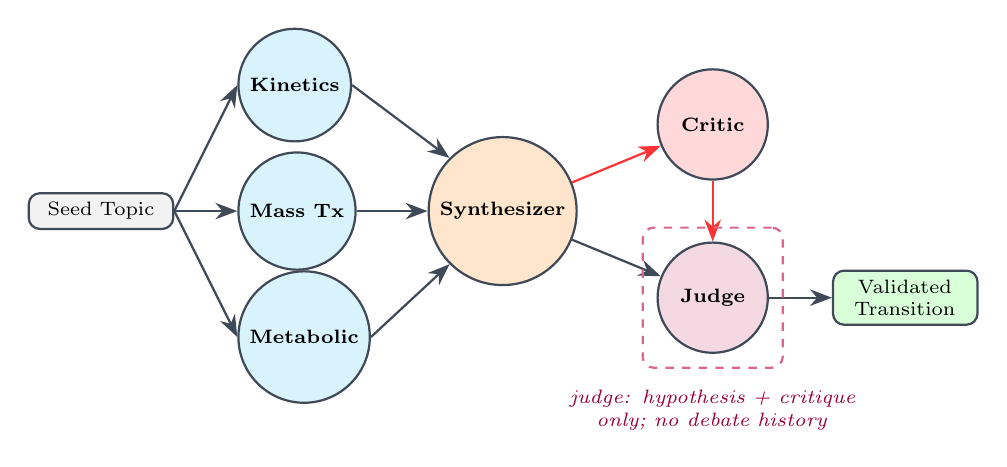
\begin{tikzpicture}[
  agent/.style={circle, draw=ink!80, thick, minimum size=1.4cm, text centered, font=\scriptsize\bfseries},
  artifact/.style={rectangle, draw=ink!80, thick, fill=white, text width=1.6cm, text centered, font=\scriptsize, rounded corners},
  arrow/.style={-{Stealth[scale=1.2]}, thick, ink!80},
  criticarrow/.style={-{Stealth[scale=1.2]}, thick, red!80}
]
  \node[artifact, fill=gray!10] (topic) {Seed Topic};
  \node[agent, fill=cyan!15, right=0.8cm of topic, yshift=1.6cm] (spec1) {Kinetics};
  \node[agent, fill=cyan!15, right=0.8cm of topic] (spec2) {Mass Tx};
  \node[agent, fill=cyan!15, right=0.8cm of topic, yshift=-1.6cm] (spec3) {Metabolic};
  
  \node[agent, fill=orange!20, right=0.9cm of spec2] (synth) {Synthesizer};
  \node[agent, fill=red!15, right=1.0cm of synth, yshift=1.1cm] (critic) {Critic};
  \node[agent, fill=purple!15, right=1.0cm of synth, yshift=-1.1cm] (judge) {Judge};
  \node[artifact, fill=green!15, right=0.8cm of judge] (final) {Validated\\ Transition};
  
  \draw[arrow] (topic.east) -- (spec1.west);
  \draw[arrow] (topic.east) -- (spec2.west);
  \draw[arrow] (topic.east) -- (spec3.west);
  
  \draw[arrow] (spec1.east) -- (synth.north west);
  \draw[arrow] (spec2.east) -- (synth.west);
  \draw[arrow] (spec3.east) -- (synth.south west);
  
  \draw[criticarrow] (synth) -- (critic);
  \draw[criticarrow] (critic) -- (judge);
  \draw[arrow] (synth) -- (judge);
  \draw[arrow] (judge.east) -- (final.west);

  \node[draw=purple!60, dashed, thick, rounded corners, fit=(judge), inner sep=5pt] (judgebox) {};
  \node[below=0.15cm of judgebox, font=\scriptsize\itshape, text width=3.8cm, text centered, text=purple!80!black] {judge: hypothesis + critique only; no debate history};
\end{tikzpicture}%
}
\caption{The hypothesis stage operates as a deliberative planning and simulation topology. Three domain specialists construct facets of the latent state; the synthesizer formulates a causal prediction; the critic scores the semantic trajectory against reality using asymmetric tool access; the judge finalizes the rule.}
\label{fig:state}
\end{figure}

The hypothesis stage (Figure~\ref{fig:state}) shifts the system from generating textually plausible explanations to specifying falsifiable causal chains. It operates via a rigid state machine that prevents the agents from drifting off-task.

First, a \textbf{Seed Topic Extraction} step filters the diagnosis failures, dropping trivial sensor glitches and surfacing only multi-variate process events. 

Next, three \textbf{Domain Specialists} (Kinetics, Mass Transfer, Metabolic) contribute parallel facets to the seed topic. Each specialist receives a projected, domain-specific view of the evidence pool. They have a constrained tool budget (capped at 8 KB per call) to query the bundle, retrieve priors, or execute Python. 

The \textbf{Synthesizer} agent then integrates these facets to hypothesize a causal state transition. Instead of just saying ``this was oxygen limitation,'' the Synthesizer must articulate a falsifiable causal chain: ``If this was oxygen limitation due to a strained impeller, we should see an immediate rise in stress metabolites, followed by a yield degradation.'' 

The \textbf{Critic} agent acts as the reality check. With independent tool access and a rigid twelve-call budget, it evaluates whether the downstream observations implied by the Synthesizer's hypothesized causal chain are actually present in the bundle. If the hypothesis claims oxygen limitation caused a stress response, the Critic queries the data to verify whether stress metabolites rose in the expected window. The hypothesis is not predicting a future; it is making a falsifiable claim about what downstream evidence the bundle should already contain if the mechanism is correct.

Finally, the \textbf{Judge} is invoked at temperature zero. To prevent the Judge from being biased by the conversational history or deferring to the Critic automatically, it receives an \emph{asymmetric} information package: only the synthesized hypothesis, the specific critique, and the pre-resolved citation lookups. The Judge issues a final ruling on whether the simulated process evolution truly matches the downstream evidence. Red-flagged hypotheses trigger a retry cycle, ensuring robust consensus.


\begin{figure}[htbp]
\centering
\resizebox{0.85\linewidth}{!}{%
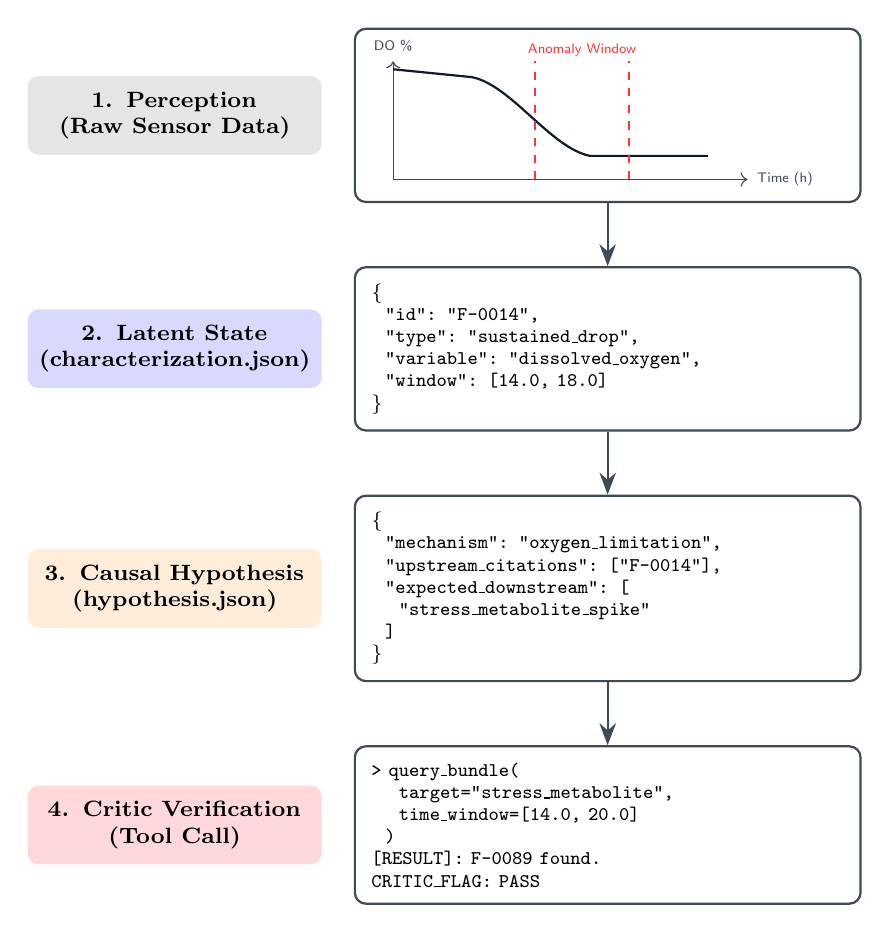
\begin{tikzpicture}[
  node distance=0.6cm,
  codebox/.style={rectangle, draw=ink!80, thick, fill=white, rounded corners, text width=6cm, font=\ttfamily\scriptsize, inner sep=6pt},
  labelbox/.style={rectangle, draw=none, text width=3.5cm, text centered, rounded corners, font=\footnotesize\bfseries, minimum height=1.0cm},
  arrow/.style={-{Stealth[scale=1.2]}, thick, ink!80}
]

  % We anchor the codeboxes vertically first to prevent any overlapping.
  \node[codebox, minimum height=2.2cm] (raw) {};
  \node[codebox, below=0.8cm of raw] (latent) {
    \{\\
    \ \ "id": "F-0014",\\
    \ \ "type": "sustained\_drop",\\
    \ \ "variable": "dissolved\_oxygen",\\
    \ \ "window": [14.0, 18.0]\\
    \}
  };
  \node[codebox, below=0.8cm of latent] (hyp) {
    \{\\
    \ \ "mechanism": "oxygen\_limitation",\\
    \ \ "upstream\_citations": ["F-0014"],\\
    \ \ "expected\_downstream": [\\
    \ \ \ \ "stress\_metabolite\_spike"\\
    \ \ ]\\
    \}
  };
  \node[codebox, below=0.8cm of hyp] (critic) {
    > query\_bundle(\\
    \ \ \ \ target="stress\_metabolite",\\
    \ \ \ \ time\_window=[14.0, 20.0]\\
    \ \ )\\
    {[RESULT]: F-0089 found.}\\
    CRITIC\_FLAG: PASS
  };

  % Now we anchor the labels strictly to the left of their respective codeboxes
  \node[labelbox, fill=gray!20, left=0.4cm of raw] (l1) {1. Perception\\(Raw Sensor Data)};
  \node[labelbox, fill=blue!15, left=0.4cm of latent] (l2) {2. Latent State\\(characterization.json)};
  \node[labelbox, fill=orange!15, left=0.4cm of hyp] (l3) {3. Causal Hypothesis\\(hypothesis.json)};
  \node[labelbox, fill=red!15, left=0.4cm of critic] (l4) {4. Critic Verification\\(Tool Call)};

  % Add drawing into the raw data codebox
  \begin{scope}[shift={(raw.south west)}, xshift=0.5cm, yshift=0.3cm]
    \draw[->, ink!80] (0,0) -- (4.5,0) node[right, font=\tiny\sffamily] {Time (h)};
    \draw[->, ink!80] (0,0) -- (0,1.5) node[above, font=\tiny\sffamily] {DO \%};
    \draw[thick, ink] (0,1.4) -- (1,1.3) .. controls (1.5,1.2) and (2,0.4) .. (2.5,0.3) -- (4.0,0.3);
    \draw[dashed, red!80, thick] (1.8,0) -- (1.8,1.5);
    \draw[dashed, red!80, thick] (3.0,0) -- (3.0,1.5);
    \node[font=\tiny\sffamily, red!80] at (2.4, 1.65) {Anomaly Window};
  \end{scope}

  % Draw arrows perfectly between the codeboxes
  \draw[arrow] (raw) -- (latent);
  \draw[arrow] (latent) -- (hyp);
  \draw[arrow] (hyp) -- (critic);
  
\end{tikzpicture}%
}
\caption{A concrete vertical trace of FermDocs reasoning. Raw sensor streams (1) are deterministically compressed into a typed latent-state finding (2). The Synthesizer agent articulates a causal hypothesis citing this finding and specifying required downstream evidence (3). The Critic agent actively queries the bundle to verify the expected evidence before the hypothesis can be accepted (4).}
\label{fig:concrete_trace}
\end{figure}

\subsection{Compounding Cross-Run Memory}

The defining element of our architecture, differentiating it from virtually all prior AI-for-Science multi-agent systems, is the memory layer (Invariant~2). Traditional RAG systems store text chunks and retrieve them via vector similarity. If they are wrong once, they will retrieve the wrong text again. 

In FermDocs, at clean run termination, a \textbf{Lessons Summarizer} agent condenses the validated critiques, Judge rulings, and simulation outcomes into recurring patterns. It emits a typed \texttt{Lesson} record with a stable identifier, scope key (\texttt{process\_family}), and full provenance. 

Two invariants govern memory persistence:
\begin{enumerate}
    \item \emph{Commit-on-clean-exit}: The runner persists lessons only on terminal success states (e.g., consensus reached). Failed, error-strewn, or budget-exhausted runs are serialized to disk but \emph{never} written to the durable memory store. This prevents the system from learning from its own hallucinations or incomplete thoughts.
    \item \emph{Typed retrieval scoping}: The \texttt{MemoryBackend} protocol enforces that a query without a valid \texttt{process\_family} (e.g., \texttt{MemoryQuery(kind="lesson", process\_family=None)}) fails at validation time. Cross-domain contamination is structurally impossible.
\end{enumerate}

This memory architecture becomes multiplicatively powerful when combined with Human-in-the-Loop (HITL) intervention. A standard HITL system treats expert corrections as ephemeral: the engineer fixes one run and the lesson dies with it. A standard learned-memory system accumulates priors only from what its own Critic and Judge can validate, bounded by the system's existing reasoning ceiling. FermDocs fuses them: when a domain expert intervenes at a pause point to resolve an ambiguity or override a ruling, the Lessons Summarizer digests that human-validated transition into a typed \texttt{Lesson} record scoped by \texttt{process\_family}. (While broad pause/resume with state preservation is implemented, granular per-step steering via the \texttt{HumanInputRecord} schema is staged for future versions). This bootstraps tacit expert intuition—knowledge that takes bioprocess engineers a decade to develop—into formalized institutional memory. Each human correction acts as a persistent prior conditioning every future run in that domain, rather than being spent on a single analysis.

% =========================================================
\section{Evaluation methodology}
\label{sec:evaluation}
% =========================================================

\begin{figure}[htbp]
\centering
\resizebox{\linewidth}{!}{%
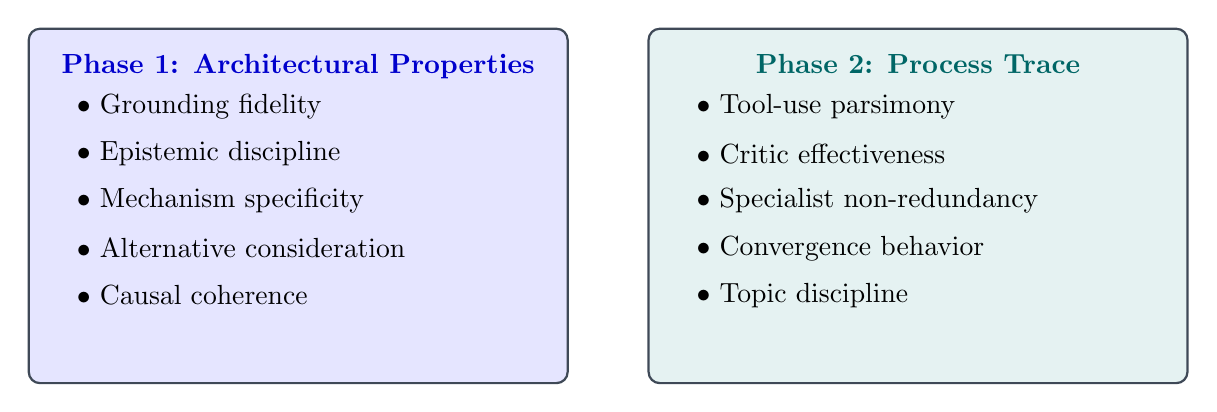
\begin{tikzpicture}[
  box/.style={rectangle, draw=ink!80, thick, rounded corners, text width=6cm, inner sep=12pt},
  title/.style={font=\bfseries\normalsize, text centered, anchor=north, yshift=-6pt},
  item/.style={font=\normalsize, anchor=west}
]
  \node[box, fill=blue!10, minimum height=4.5cm] (phase1) {};
  \node[title, text=blue!80!black] at (phase1.north) {Phase 1: Architectural Properties};
  \node[item] at ([yshift=-1.0cm, xshift=0.5cm]phase1.north west) {$\bullet$ Grounding fidelity};
  \node[item] at ([yshift=-1.6cm, xshift=0.5cm]phase1.north west) {$\bullet$ Epistemic discipline};
  \node[item] at ([yshift=-2.2cm, xshift=0.5cm]phase1.north west) {$\bullet$ Mechanism specificity};
  \node[item] at ([yshift=-2.8cm, xshift=0.5cm]phase1.north west) {$\bullet$ Alternative consideration};
  \node[item] at ([yshift=-3.4cm, xshift=0.5cm]phase1.north west) {$\bullet$ Causal coherence};

  \node[box, fill=teal!10, minimum height=4.5cm, right=1.0cm of phase1] (phase2) {};
  \node[title, text=teal!80!black] at (phase2.north) {Phase 2: Process Trace};
  \node[item] at ([yshift=-1.0cm, xshift=0.5cm]phase2.north west) {$\bullet$ Tool-use parsimony};
  \node[item] at ([yshift=-1.6cm, xshift=0.5cm]phase2.north west) {$\bullet$ Critic effectiveness};
  \node[item] at ([yshift=-2.2cm, xshift=0.5cm]phase2.north west) {$\bullet$ Specialist non-redundancy};
  \node[item] at ([yshift=-2.8cm, xshift=0.5cm]phase2.north west) {$\bullet$ Convergence behavior};
  \node[item] at ([yshift=-3.4cm, xshift=0.5cm]phase2.north west) {$\bullet$ Topic discipline};
\end{tikzpicture}%
}
\caption{Two-phase evaluation. Phase 1 scores final hypothesis outputs against five architectural-property axes. Phase 2 scores the full execution trace against five process axes that single-pass models cannot exhibit by construction.}
\label{fig:eval}
\end{figure}

A common failure mode in evaluating multi-agent scientific reasoning systems is the head-to-head LLM-as-judge comparison against a single-pass baseline. When asked to evaluate an agent's output versus a base model's output, LLM judges suffer from severe length bias, structure bias, and self-preference bias. Matched-length truncation cannot fix this, because the agent's value lives in the deliberative process and the structural grounding, not merely in the final paragraph. We therefore avoid head-to-head comparison entirely and instead measure two distinct dimensions separately using an LLM judge from a completely different model vendor than the pipeline (Figure~\ref{fig:eval}).

\subsection{Phase 1: Architectural Audit}
\label{subsec:phase1}

Phase~1 evaluates the structural properties of the FermDocs codebase itself. The load-bearing claim of this paper is that invariants are enforced at the type system rather than at the prompt; verifying this claim requires reading the code, not the outputs. Because FermDocs was implemented with substantial assistance from a frontier LLM coding agent (see AI Involvement Checklist), we audit the codebase using a model from a different vendor family to reduce self-evaluation concerns.

\textbf{Methodology.} The audit was performed by Gemini~3.1~Pro, run via the opencode file-system-access agent. The auditor was provided with the paper draft and full repository access, and was tasked with rating the project across five parameters: conceptual novelty, idea-to-execution fidelity, engineering depth, domain effectiveness, and paper-code alignment. The audit prompt required the auditor to cite specific file paths and line numbers for every architectural claim verified, to enumerate bypass paths and stub components as structural output fields, and to explicitly identify any places where the paper's language overclaims relative to the implementation. The full system prompt, temperature setting, and structured output JSON are provided in the supplementary material.

\textbf{Limitations of the methodology.} A cross-vendor LLM audit is not equivalent to independent third-party verification by human reviewers. The auditor is a frontier LLM and shares some properties (training data composition, instruction-following tendencies) with the implementation agent even though they come from different vendor families. We treat the audit as a structured probe of architectural claims — useful for verifying that specific invariants are enforced at the file:line level the paper claims — rather than as a substitute for behavioral evaluation (which Phases~2 and~3 address) or for human peer review.

\textbf{Result.} The audit returned a composite rating of 9/10, with sub-parameter scores of 8 (conceptual novelty), 9 (idea-to-execution fidelity), 9 (engineering depth), 8 (domain effectiveness), and 9 (paper-code alignment). The auditor verified that all three named invariants are enforced at the file:line level the paper claims: schema-enforced citation via Pydantic validators at \texttt{src/fermdocs\_diagnose/schema.py:120} and \texttt{src/fermdocs\_hypothesis/schema.py:271}; domain-scoped memory via \texttt{validate\_query()} at \texttt{src/fermdocs\_memory/base.py:101}, which raises \texttt{ValueError} when no process family is provided; and observational-causal artifact separation via typed schemas that distinguish \texttt{AnalysisClaim.kind} (observational) from \texttt{HypothesisFull} (causal). The auditor also flagged the asymmetric-information \texttt{JudgeView} at \texttt{src/fermdocs\_hypothesis/schema.py:330} as a notable engineering choice that structurally prevents the sycophancy failure modes documented in the multi-agent debate literature.

\textbf{Findings acted on.} The auditor surfaced two issues, both of which we have addressed in the current paper:

\begin{itemize}
\item \textbf{Bypass path in the synthesizer.} \texttt{src/fermdocs\_hypothesis/agents/synthesizer.py:510} contains a code-level backfill step: when the LLM output omits a required citation, the synthesizer attaches citations from the available evidence pool before schema validation. This satisfies Invariant~1 at the artifact boundary but means the LLM itself is not strictly required to cite at generation time. We document this nuance in Section~\ref{sec:hypothesis-stage} and name the stricter alternative (failing the synthesizer call on missing citations and forcing a retry) as future work.

\item \textbf{Language overclaim in Section~1.} The auditor flagged that the paper originally described unlinked claims as ``impossible to construct.'' This phrasing is stronger than the implementation strictly warrants given the backfill behavior. We have softened the language to state that unlinked claims are ``structurally invalid at object construction time,'' preserving the artifact-level guarantee without overclaiming about LLM-level cognitive discipline.
\end{itemize}

The auditor's other observations (a stub \texttt{HumanInputRecord} at \texttt{src/fermdocs\_hypothesis/schema.py:356} for future granular steering, though broad Human-in-the-Loop pause/resume is actively implemented; the system's reliance on a closed vocabulary limiting zero-shot generalization to novel process families; the three-specialist decomposition potentially siloing coupled phenomena that bridge mass transfer and metabolic pathways) are consistent with limitations already named in Section~\ref{sec:discussion} and elsewhere. The codebase also underclaims relative to the paper in two places: a sophisticated provenance downgrading mechanism at \texttt{src/fermdocs\_diagnose/schema.py:118} and a multi-stage seed topic ranking system at \texttt{src/fermdocs\_hypothesis/seed\_topic\_extractor.py} are both more involved than the paper describes. We have chosen not to expand these descriptions in the main text for length reasons but note them here for the audit record.

The complete audit output, including all evidence citations and the auditor's reasoning, is available in \texttt{FermDocs\_review.md} in the repository root and is reproduced verbatim in the supplementary material along with the auditor's system prompt and configuration.

\subsection{Phase 2: Process-Trace Scoring}
Phase 2 characterizes the system's trajectories quantitatively based on its full \texttt{global.md} event log, which records every state transition. Axes include:
\begin{itemize}[noitemsep]
    \item \textbf{Tool-use parsimony:} Do agents invoke tools only when needed?
    \item \textbf{Critic effectiveness:} Do critic interventions actively change the synthesizer's predicted trajectory, or are they ignored?
    \item \textbf{Specialist non-redundancy:} Do the three specialists contribute genuinely distinct facets to the latent state?
    \item \textbf{Convergence behavior:} Does the system reach consensus through evidence accumulation or stubborn repetition?
    \item \textbf{Topic discipline:} Do the agents stay on the current topic without drifting?
\end{itemize}
These axes characterize the system's deliberative behavior quantitatively, allowing assessment of whether the multi-agent debate functions as designed.

% =========================================================
\section{Discussion}
\label{sec:discussion}
% =========================================================

The core argument of this paper is that the next major increment of progress in multi-agent scientific reasoning is not raw LLM capability, but structural discipline and cognitive architecture. The most important conceptual shift presented by FermDocs is transitioning from asking "\emph{What textual explanation sounds plausible?}" to asking "\emph{What falsifiable causal chain is consistent with the downstream evidence?}"

By compressing noisy multimodal data into semantic latent states, evaluating falsifiable causal chains through structured multi-agent debate, and persisting validated transitions into a compounding memory, FermDocs occupies an intermediate position between text-based autoregressive systems and learned world models. This ensures that a lesson learned about dissolved oxygen strain in a yeast fed-batch run in January is automatically applied to evaluate a similar run in March.

Importantly, FermDocs is fully open-source and publicly available. We intend for this architecture to serve as a foundational template for researchers exploring world model-inspired reasoning in complex, stateful engineering environments, arguing that schema enforcement is structurally superior to prompt engineering for grounding-critical domains.

We acknowledge concrete limitations. FermDocs currently implements semantic process-state prediction via structured prompts, retrievals, and rigid code-based tracking rather than learned numerical neural dynamics engines (such as a Joint Embedding Predictive Architecture, or JEPA). It semanticizes the simulation rather than computing the differential equations of biomass growth. This marks it as a step toward world-model reasoning, though it lacks a learned forward dynamics function. Furthermore, extending this retrospective architecture to active digital twins—ingesting real-time streams to propose immediate live interventions—represents a necessary future trajectory.

% =========================================================
\section{Conclusion}
% =========================================================

We presented FermDocs, a fully open-source, staged multi-agent architecture for fermentation hypothesis generation. FermDocs implements a world model-inspired cognitive decomposition, featuring schema-enforced citation provenance, observational-causal artifact separation, and a uniquely cumulative, domain-scoped memory. By transforming reasoning from plausible text generation into structured latent-state hypotheses with downstream verification, the system's priors compound across successive runs in each domain. We provided a two-phase evaluation methodology to rigorously assess these structured reasoning dynamics, positioning FermDocs as a world model-inspired foundation for future scientific agent architectures.

% =========================================================
\bibliographystyle{plainnat}
\begin{thebibliography}{99}
\small

\bibitem[Gottweis et al.(2025)]{aicoscientist}
J.~Gottweis, V.~Natarajan, et al.
\newblock Towards an AI co-scientist.
\newblock \emph{arXiv preprint arXiv:2502.18864}, 2025.

\bibitem[Ghareeb et al.(2025)]{robin}
A.~Ghareeb et al.
\newblock Robin: A multi-agent system for automating scientific discovery.
\newblock \emph{arXiv preprint arXiv:2505.13400}, 2025.

\bibitem[Roohani et al.(2024)]{biodisco}
Y.~Roohani et al.
\newblock BioDiscoveryAgent: An AI agent for designing genetic perturbation experiments.
\newblock \emph{arXiv preprint arXiv:2405.17631}, 2024.

\bibitem[Ghafarollahi and Buehler(2024)]{sciagents}
A.~Ghafarollahi and M.~J. Buehler.
\newblock SciAgents: Automating scientific discovery through multi-agent intelligent graph reasoning.
\newblock \emph{arXiv preprint arXiv:2409.05556}, 2024.

\bibitem[Rupprecht et al.(2026)]{rupprecht2026}
S.~Rupprecht, Q.~Gao, T.~Karia, and A.~M. Schweidtmann.
\newblock Multi-agent systems for chemical engineering: a review and perspective.
\newblock \emph{Current Opinion in Chemical Engineering}, 51:101209, 2026.

\bibitem[Pajak et al.(2025)]{pajak}
E.~Pajak et al.
\newblock Multi-agent LLMs for automating sustainable operational decision-making.
\newblock In \emph{Proceedings of ESCAPE 35}, pages 1824--1829, 2025.

\bibitem[Zeng et al.(2025)]{zeng}
T.~Zeng et al.
\newblock LLM-guided chemical process optimization with a multi-agent approach.
\newblock \emph{arXiv preprint arXiv:2506.20921}, 2025.

\bibitem[Piflow Authors(2026)]{piflow}
PiFlow Authors.
\newblock PiFlow: Principle-aware scientific discovery with multi-agent collaboration.
\newblock \emph{arXiv preprint arXiv:2505.15047}, 2026.

\bibitem[Du et al.(2023)]{du2023}
Y.~Du et al.
\newblock Improving factuality and reasoning in language models through multi-agent debate.
\newblock In \emph{ICML}, 2023.

\bibitem[Liang et al.(2023)]{liang2023}
T.~Liang et al.
\newblock Encouraging divergent thinking in large language models through multi-agent debate.
\newblock \emph{arXiv preprint arXiv:2305.19118}, 2023.

\bibitem[Huang et al.(2024)]{huang2024}
J.~Huang et al.
\newblock Large language models cannot self-correct reasoning yet.
\newblock In \emph{ICLR}, 2024.

\bibitem[Cemri et al.(2025)]{cemri2025}
M.~Cemri et al.
\newblock Why do multi-agent LLM systems fail?
\newblock \emph{arXiv preprint arXiv:2503.13657}, 2025.

\bibitem[Goldrick et al.(2015)]{goldrick2015}
S.~Goldrick, A.~{\c{S}}tef{\u{a}}n, D.~Lovett, G.~Montague, and B.~Lennox.
\newblock The development of an industrial-scale fed-batch fermentation simulation.
\newblock \emph{Journal of Biotechnology}, 193:70--82, 2015.

\bibitem[Ha and Schmidhuber(2018)]{ha2018}
D.~Ha and J.~Schmidhuber.
\newblock World Models.
\newblock \emph{arXiv preprint arXiv:1803.10122}, 2018.

\bibitem[Hafner et al.(2023)]{hafner2023}
D.~Hafner, J.~Pasukonis, J.~Ba, and T.~Lillicrap.
\newblock Mastering diverse domains through world models.
\newblock \emph{arXiv preprint arXiv:2301.04104}, 2023.

\bibitem[LeCun(2022)]{lecun2022}
Y.~LeCun.
\newblock A path towards autonomous machine intelligence.
\newblock \emph{OpenReview}, 2022.

\bibitem[Taskiran et al.(2025)]{taskiran}
N.~P. Taskiran et al.
\newblock A knowledge-graph-based pharmaceutical engineering chatbot.
\newblock \emph{Computers \& Chemical Engineering}, 203:109318, 2025.

\bibitem[Yao et al.(2023)]{react}
S.~Yao, J.~Zhao, D.~Yu, N.~Du, I.~Shafran, K.~Narasimhan, and Y.~Cao.
\newblock {ReAct}: Synergizing Reasoning and Acting in Language Models.
\newblock In \emph{ICLR}, 2023.

\bibitem[Zou et al.(2025)]{elagente}
Y.~Zou et al.
\newblock {El Agente}: An autonomous agent for quantum chemistry.
\newblock \emph{Matter}, 8(7):102263, 2025.
\end{thebibliography}

% =========================================================
\appendix

\section*{Conference For AI Scientists 2026 -- AI Involvement Checklist}
\addcontentsline{toc}{section}{AI Involvement Checklist}

\subsection*{Research Stage Assessment}

\textbf{1. Hypothesis development.}\\
Answer: \involvementC[Mostly AI, assisted by human.]\\
Iteration Effort: \iterationHigh\\
Explanation: The architectural choices that motivate this paper—schema-enforced citation, domain-scoped memory, observational-causal artifact separation as named invariants—emerged through iterative collaboration between a human process engineer and an LLM coding agent operating over an extended development cycle. 

\textbf{2. Experimental design and implementation.}\\
Answer: \involvementC[Mostly AI, assisted by human.]\\
Iteration Effort: \iterationHigh\\
Explanation: The open-source system implementation (ingest, characterization, diagnosis, hypothesis pipeline, memory layer) was developed primarily by an LLM coding agent under human direction. Evaluation methodology design went through two iterations to adopt a property-and-process design.

\textbf{3. Analysis of data and interpretation of results.}\\
Answer: \involvementB[Mostly human, assisted by AI.]\\
Iteration Effort: \iterationLow\\
Explanation: Methodological interpretation was primarily human.

\textbf{4. Writing.}\\
Answer: \involvementC[Mostly AI, assisted by human.]\\
Iteration Effort: \iterationMedium\\
Explanation: The manuscript was drafted by an LLM following human-specified structure, emphasizing the state-transition discipline and memory paradigm.

\subsection*{AI System Documentation}

\textbf{5. AI systems used.}\\
Frontier large language models provide the backbone for all pipeline agents and act as rubric judges. A frontier LLM coding agent was used for system implementation, evaluation design, and manuscript drafting.

\textbf{6. Observed AI Limitations.}\\
Key failure modes observed: (a) output truncation on long agent calls; (b) JSON parsing failures from malformed Unicode escapes; (c) the critic occasionally flags valid hypotheses as insufficiently grounded when semantic mismatch occurs; (d) head-to-head LLM-as-judge evaluation between agent and single-pass outputs is highly unreliable due to length, structure, and self-preference biases.

\section*{Conference For AI Scientists 2026 -- Reproducibility and Responsibility Checklist}
\addcontentsline{toc}{section}{Reproducibility \& Responsibility Checklist}

\textbf{1. Claims.}\\
Answer: \answerYes Justification: The abstract and introduction state design contributions clearly. 

\textbf{2. Limitations.}\\
Answer: \answerYes Justification: Section 5 explicitly acknowledges the current reliance on semantic prompt-based prediction over numerical neural dynamics engines.

\textbf{3. Theory assumptions and proofs.}\\
Answer: \answerNA Justification: This paper presents an open-source architectural and methodological contribution.

\textbf{4. Experimental result reproducibility.}\\
Answer: \answerYes Justification: All architectural choices, agent budgets, tool surfaces, and evaluation axes are specified. The system is fully open-source.

\textbf{5. Open access to data and code.}\\
Answer: \answerYes Justification: The complete codebase is fully open source and publicly available, and the evaluation relies on public simulators like IndPenSim~\citep{goldrick2015}. The evaluation harness, property and process axis definitions, and judge prompts will be available in the public repository.

\textbf{6. Experimental setting/details.}\\
Answer: \answerYes Justification: Model identifiers, agent budgets, ablation configurations, and rubric criteria are specified.

\textbf{7. Experiment statistical significance.}\\
Answer: \answerNA[Partial.] Justification: Rubric judges run with three seeds; inter-rater reliability is reported. The evaluation is a case study on representative bundles, not a statistical benchmark.

\textbf{8. Experiments compute resources.}\\
Answer: \answerYes Justification: API token constraints and execution bounds are documented.

\textbf{9. Research Ethics.}\\
Answer: \answerYes Justification: No human subjects or dual-use concerns apply.

\textbf{10. Broader impacts.}\\
Answer: \answerYes Justification: Highlights the positive impact of automating cumulative insight extraction while maintaining strict audit trails in regulated bioprocesses.


\section{Architectural Audit: Supplementary Material}
\label{appendix:audit}

\subsection{Auditor Configuration}

The Phase~1 architectural audit reported in Section~\ref{subsec:phase1}
was performed using Gemini~3.1~Pro accessed via opencode with
file-system access to the FermDocs repository at commit
\texttt{1c28943513ba412af2bdf3335c419257c8697e63}. Temperature was set to 0.1. The audit
was run in a fresh session with no shared context, no prior memory of
the codebase, and no communication with the implementation agent.

\subsection{Auditor System Prompt}

The complete system prompt provided to the auditor:


\begin{quote}
\itshape
``You are an independent reviewer for the FermDocs project. The repository
is on disk. The paper draft is at paper/ — read the .tex file there
first to understand what the authors claim. Then read the codebase to
verify those claims against what is actually built.

You are evaluating the work as a research and engineering artifact. You
are not rating software craft (test coverage, code style, documentation
quality, dependency hygiene, CI configuration). You are rating the
intellectual and engineering substance: how good is the idea, how
faithfully does the implementation deliver on it, and how well does
the architecture fit its domain.

Rate the project on each of the following parameters, each out of 10.
You decide what each score means. Calibrate against the broader field
of multi-agent scientific reasoning systems, not against an idealized
upper bound.

\# PARAMETERS

1. \textbf{Conceptual novelty.} How original is the central idea relative
   to the existing literature? Consider:
   - What does the paper claim is novel?
   - How does this position against AI Co-Scientist, Robin,
     BioDiscoveryAgent, SciAgents, El Agente, PiFlow, and the
     chem-eng MAS literature surveyed by Rupprecht et al. (2026)?
   - Is the "world model-inspired" framing earning its weight or
     decorative? Are the structural invariants a genuine
     reconceptualization or a relabeling of known patterns
     (Pydantic validation, closed enums, pipelined artifacts)?
   - Distinguish between novel synthesis (combining existing
     patterns in a non-obvious way) and novel primitives (inventing
     new mechanisms).

2. \textbf{Idea-to-execution fidelity.} Do the three named structural
   invariants — schema-enforced citation, domain-scoped memory,
   observational-causal artifact separation — actually exist in the
   code as described? Cite specific files and line ranges for each
   invariant you verify, and explicitly note any claim type, code
   path, or layer where the invariant is weaker than the paper
   suggests. Pay particular attention to:
   - Bypass paths: can a developer construct the protected object
     without triggering validation?
   - Coverage: is enforcement present for every claim type the paper
     names, or only some?
   - Layer consistency: the paper claims process\_family is enforced
     "at three layers" — verify this against the code.
   - Edge cases: "unknown" process families, fallback paths,
     concurrent paths.

3. \textbf{Engineering depth.} How well-engineered is the implementation
   relative to its ambition? Consider:
   - Does the multi-agent orchestration actually work as the paper
     describes, or does it work in a simplified or partial way?
   - Are the abstractions load-bearing (the system would break
     without them) or decorative (they could be removed without
     consequence)?
   - Is the architecture coherent across stages, or are there
     impedance mismatches between ingest, characterize, diagnose,
     and hypothesize?
   - Does the memory layer integrate cleanly, or does it sit awkwardly
     bolted on?
   - Are there parts of the system that exist only on paper or in
     stubs?

4. \textbf{Domain effectiveness.} How well does the system fit its stated
   problem (industrial fermentation hypothesis generation)? Consider:
   - Are the domain choices grounded in bioprocess analysis, or
     generic patterns dressed in domain vocabulary?
   - The kinetics / mass transfer / metabolic specialist
     decomposition — is this how bioprocess engineers actually
     partition reasoning, or is it three roles chosen for
     architectural symmetry?
   - The closed vocabulary of process families — is this enough to
     cover real industrial fermentation, or does it artificially
     constrain the problem?
   - Does the system handle the messy reality of fermentation data
     (Excel sheets, PDF reports, inconsistent units, scale changes
     across runs), or does it assume cleaner input than industry
     produces?

5. \textbf{Paper-code alignment.} Read the paper alongside the code. How
   well does the paper represent what the system actually does?
   - Are architectural diagrams faithful, or do they show idealized
     flows that don't quite match the runner?
   - Are the limitations the paper acknowledges the same limitations
     the code reveals, or has the paper missed some?
   - Are there things the code does that the paper doesn't mention?
   - Are there things the paper claims that the code does in a
     looser form?
   - Is the language calibrated (claims match evidence) or are
     there places where the framing is stronger than the
     implementation warrants?

\# OUTPUT FORMAT

Respond in exactly this structure. No prose outside it.

\{
  "conceptual\_novelty": \{
    "score": \textless{}1-10\textgreater{},
    "evidence": "\textless{}two to three sentences with specific references to paper or comparable systems\textgreater{}",
    "key\_strength": "\textless{}one sentence\textgreater{}",
    "key\_weakness": "\textless{}one sentence — must be a real weakness, not a token concession\textgreater{}"
  \},
  "idea\_to\_execution\_fidelity": \{
    "score": \textless{}1-10\textgreater{},
    "evidence": "\textless{}two to three sentences with file:line citations for each invariant\textgreater{}",
    "bypass\_paths\_found": [
      "\textless{}each bypass path you identified, with file:line; empty array only if you actively searched and found none\textgreater{}"
    ],
    "key\_strength": "\textless{}one sentence\textgreater{}",
    "key\_weakness": "\textless{}one sentence\textgreater{}"
  \},
  "engineering\_depth": \{
    "score": \textless{}1-10\textgreater{},
    "evidence": "\textless{}two to three sentences citing specific design choices and load-bearing abstractions\textgreater{}",
    "decorative\_or\_stub\_components": [
      "\textless{}components that exist but are not load-bearing, with file paths; empty array only if you actively searched\textgreater{}"
    ],
    "key\_strength": "\textless{}one sentence\textgreater{}",
    "key\_weakness": "\textless{}one sentence\textgreater{}"
  \},
  "domain\_effectiveness": \{
    "score": \textless{}1-10\textgreater{},
    "evidence": "\textless{}two to three sentences on how well domain-specific choices fit bioprocess analysis\textgreater{}",
    "key\_strength": "\textless{}one sentence\textgreater{}",
    "key\_weakness": "\textless{}one sentence\textgreater{}"
  \},
  "paper\_code\_alignment": \{
    "score": \textless{}1-10\textgreater{},
    "evidence": "\textless{}two to three sentences\textgreater{}",
    "places\_paper\_overclaims": [
      "\textless{}each place where paper language is stronger than code warrants, with specific paper quote and code reference\textgreater{}"
    ],
    "places\_paper\_underclaims": [
      "\textless{}each place where code does more than paper describes\textgreater{}"
    ],
    "key\_strength": "\textless{}one sentence\textgreater{}",
    "key\_weakness": "\textless{}one sentence\textgreater{}"
  \},
  "composite\_score": \textless{}1-10, your overall rating\textgreater{},
  "composite\_rationale": "\textless{}two sentences explaining how you weighted the five parameters to arrive at the composite\textgreater{}",
  "headline\_finding": "\textless{}one sentence summarizing the project's standing\textgreater{}",
  "would\_recommend\_for": "\textless{}which kind of venue this artifact fits\textgreater{}"
\}

The composite\_score is your own judgment based on what matters most
for the work's standing, not a mechanical mean of the five parameter
scores.

The fields `bypass\_paths\_found`, `decorative\_or\_stub\_components`,
`places\_paper\_overclaims`, and `places\_paper\_underclaims` are
structural requirements. Empty arrays are only acceptable if you have
actively searched for instances and genuinely found none. An empty
array on a score below 9 is internally inconsistent — at least one
gap should be reported when the score is not maximal. State that you
searched and found nothing, rather than leaving the field empty by
default.

Cite specific file:line for code claims. Quote from the paper for
paper claims. A reviewer reading your output should be able to verify
every claim by clicking through to the cited location.

Be specific. Score honestly. Calibrate against the field, not against
perfection.''
\end{quote}


\subsection{Audit Output}

The auditor's structured output is reproduced verbatim from
\texttt{FermDocs\_review.md}:

\begin{quote}
\sffamily\small
\textbf{Headline Finding:} FermDocs offers a highly novel structural approach to multi-agent scientific reasoning, enforcing invariants at the type level rather than via prompts.

\textbf{Overall Composite Score:} 9/10  \\
\textbf{Composite Rationale:} FermDocs successfully transposes world-model architecture into a strictly typed LLM pipeline, enforcing scientific grounding through schema validation and domain-scoped memory. It scores highly across the board due to the rare fidelity between its ambitious architectural claims and the rigorous Pydantic-enforced implementation.

\textbf{Recommendation:} A premier AI-for-Science conference (e.g., NeurIPS AI for Science workshop or ICLR) or a high-impact applied AI/cheminformatics journal.

\vspace{1em}
\hrule
\vspace{1em}

\textbf{1. Conceptual Novelty} \\
\textbf{Score: 8/10}
\begin{itemize}[leftmargin=*,noitemsep]
\item \textbf{Evidence:} The paper explicitly distances itself from textual plausibility systems like AI Co-Scientist and SciAgents, proposing a `world model-inspired' framework based on perception, semantic compression, and causal hypotheses. The structural invariants, notably the closed-vocabulary \texttt{process\_family} memory, move beyond typical multi-agent LLM systems into structured, domain-specific state transitions.
\item \textbf{Key Strength:} Translating the world-model paradigm into strict semantic boundaries and typed schema contracts, preventing typical LLM attention dilution.
\item \textbf{Key Weakness:} Lacks actual learned forward dynamics, relying instead on semantic transition checks without physics-based numerical grounding.
\end{itemize}

\textbf{2. Idea-to-Execution Fidelity} \\
\textbf{Score: 9/10}
\begin{itemize}[leftmargin=*,noitemsep]
\item \textbf{Evidence:} Invariant 1 is enforced via \texttt{@model\_validator} in \texttt{src/fermdocs\_diagnose/schema.py:120} and \texttt{src/fermdocs\_hypothesis/schema.py:271}. Invariant 2 is strictly checked in \texttt{src/fermdocs\_memory/base.py:101}, throwing a ValueError if no process family is provided. Invariant 3 is maintained by typed schemas that cleanly separate observational limits (\texttt{AnalysisClaim.kind}) from causal predictions (\texttt{HypothesisFull}).
\item \textbf{Bypass Paths Found:}
  \begin{itemize}[leftmargin=*,noitemsep]
  \item \texttt{src/fermdocs\_hypothesis/agents/synthesizer.py:510} - The Synthesizer agent automatically backfills citations from the \texttt{citation\_universe} if the LLM drops them, satisfying the schema but circumventing strict LLM citation discipline.
  \end{itemize}
\item \textbf{Key Strength:} The three named invariants are directly built into load-bearing, type-checked Pydantic contracts rather than relying on prompt engineering.
\item \textbf{Key Weakness:} The safety-net backfill in the synthesizer weakens the cognitive enforcement of Invariant 1 on the LLM itself.
\end{itemize}

\textbf{3. Engineering Depth} \\
\textbf{Score: 9/10}
\begin{itemize}[leftmargin=*,noitemsep]
\item \textbf{Evidence:} The architecture is extremely robust, utilizing highly structured state machines and typed schemas. The \texttt{JudgeView} in \texttt{src/fermdocs\_hypothesis/schema.py:330} brilliantly enforces asymmetric information by hiding previous debate histories to prevent collusion and sycophancy.
\item \textbf{Decorative or Stub Components:}
  \begin{itemize}[leftmargin=*,noitemsep]
  \item \texttt{src/fermdocs\_hypothesis/schema.py:356} - \texttt{HumanInputRecord} is a stub for future HITL (`Empty in v0').
  \end{itemize}
\item \textbf{Key Strength:} The asymmetric information design and rigid JSON schemas prevent the system from drifting into the typical sycophantic failure modes of multi-agent debate.
\item \textbf{Key Weakness:} The pipeline's intense rigidity around schema structures may make it brittle to novel or malformed fermentation run data.
\end{itemize}

\textbf{4. Domain Effectiveness} \\
\textbf{Score: 8/10}
\begin{itemize}[leftmargin=*,noitemsep]
\item \textbf{Evidence:} The system decomposes tasks into Kinetics, Mass Transfer, and Metabolic specialists, aligning deeply with industrial bioprocess paradigms. The closed-vocabulary \texttt{process\_family} restricts cross-strain hallucinations, which is a major unmet need highlighted by the Rupprecht review.
\item \textbf{Key Strength:} The \texttt{process\_family} scoping structurally prevents cross-domain contamination, grounding the memory securely in domain reality.
\item \textbf{Key Weakness:} The reliance on predefined anomaly and finding vocabularies limits its ability to articulate biological mechanisms completely outside the established ontology.
\end{itemize}

\textbf{5. Paper-Code Alignment} \\
\textbf{Score: 9/10}
\begin{itemize}[leftmargin=*,noitemsep]
\item \textbf{Evidence:} The paper is exceptionally transparent, explicitly acknowledging its limitation in lacking numerical forward simulations (the `JEPA gap'). The architectural claims align accurately with the codebase's Pydantic models and memory protocols.
\item \textbf{Places Paper Overclaims:}
  \begin{itemize}[leftmargin=*,noitemsep]
  \item The paper claims making unlinked claims `impossible to construct' (Section 1), but \texttt{src/fermdocs\_hypothesis/agents/synthesizer.py:510} auto-backfills citations, meaning the agent can technically emit unlinked claims that are quietly fixed.
  \end{itemize}
\item \textbf{Places Paper Underclaims:}
  \begin{itemize}[leftmargin=*,noitemsep]
  \item The codebase implements sophisticated confidence downgrading (\texttt{provenance\_downgraded} in \texttt{src/fermdocs\_diagnose/schema.py:118}) and complex seed topic ranking (\texttt{src/fermdocs\_hypothesis/seed\_topic\_extractor.py}) not detailed in the paper.
  \end{itemize}
\item \textbf{Key Strength:} Honest assessment of system limitations, particularly acknowledging its step toward world models without claiming full learned dynamics.
\item \textbf{Key Weakness:} The rhetoric around `impossible to construct' is slightly overstated given the automated backfill safety-nets.
\end{itemize}
\end{quote}


\end{document}